%!TEX program = xelatex

\documentclass[11pt,titlepage]{report}
%!TEX root = main.tex

\usepackage[T1]{fontenc}
\usepackage{lmodern}
\usepackage[svgnames]{xcolor}
\usepackage{fontspec} % XeLaTeX required!
\usepackage{graphicx}
\usepackage{circuitikz}
\usepackage{tikz}
\usepackage{pifont}
\usepackage[some]{background}
\usepackage{xltxtra} 
\usepackage{setspace}
\usepackage[absolute]{textpos}
\usepackage[latin1]{inputenc}
\usepackage[english]{babel}
\usepackage{graphicx}
\usepackage{wrapfig}
\usepackage{fullpage}
\usepackage[margin=1in]{geometry}
\usepackage{float}
\usepackage{url}
\usepackage{multicol}
\usepackage{hyperref}
\usepackage{titlepic}
\usepackage{standalone}
\usepackage{siunitx}
\usepackage{booktabs}
\usepackage{amsmath}
\usepackage{unicode-math}
\usepackage{verbatim}
\usepackage{enumitem}
\usepackage{listings}
\usepackage{multirow}
\usepackage{pgfplots}
\pgfplotsset{compat=1.8}
\usepackage{caption} 
\usepackage[parfill]{parskip}
\usepackage{import}
\usepackage[backend=bibtexu,texencoding=utf8,bibencoding=utf8,style=ieee,sortlocale=en_GB,language=auto]{biblatex}
\usepackage[strict,autostyle]{csquotes}
\usepackage[final]{pdfpages}
\usepackage{subcaption}
\usepackage{ifplatform}
%\captionsetup[table]{skip=10pt}


% Fix for includepdf bug in Mac OS X
\newcommand{\insertpdfpath}[1]{
	\ifwindows
	\newcommand{\insertpdf}[2]{\includepdf[pages=##1]{##2}}
	\else
	\newcommand{\insertpdf}[2]{\includepdf[pages=##1]{#1/##2}}
	\fi
}

%set fonts
\setmainfont[Ligatures=TeX]{Myriad Pro}
\setmathfont{Asana Math}
\setmonofont{Lucida Console}

\usepackage{titlesec, color}
\renewcommand{\familydefault}{\sfdefault} %set font family
\renewcommand{\arraystretch}{1.2} %set table vertical spacing
\setlength\parindent{0pt} %no paragraph indent
\hypersetup{ %setup hyperlinks
    colorlinks,
    citecolor=black,
    filecolor=black,
    linkcolor=black,
    urlcolor=black
}

%redesign chapter headings
\definecolor{gray75}{gray}{0.75}
\newcommand{\chapternumber}{\thechapter}
\newcommand{\hsp}{\hspace{20pt}}
\titleformat{\chapter}[hang]{\Huge\bfseries}{\chapternumber\hsp\textcolor{gray75}{|}\hsp}{0pt}{\Huge\bfseries}

%Redefine appendix headers
\renewcommand{\appendixname}{Appendix}
\renewcommand{\appendixtocname}{Appendices}
\renewcommand{\appendixpagename}{Appendices}

%For code listings
\definecolor{black}{rgb}{0,0,0}
\definecolor{browntags}{rgb}{0.65,0.1,0.1}
\definecolor{bluestrings}{rgb}{0,0,1}
\definecolor{graycomments}{rgb}{0.4,0.4,0.4}
\definecolor{redkeywords}{rgb}{1,0,0}
\definecolor{bluekeywords}{rgb}{0.13,0.13,0.8}
\definecolor{greencomments}{rgb}{0,0.5,0}
\definecolor{redstrings}{rgb}{0.9,0,0}
\definecolor{purpleidentifiers}{rgb}{0.01,0,0.01}


\lstdefinestyle{csharp}{
language=[Sharp]C,
showspaces=false,
showtabs=false,
breaklines=true,
showstringspaces=false,
breakatwhitespace=true,
escapeinside={(*@}{@*)},
columns=fullflexible,
commentstyle=\color{greencomments},
keywordstyle=\color{bluekeywords}\bfseries,
stringstyle=\color{redstrings},
identifierstyle=\color{purpleidentifiers},
basicstyle=\ttfamily\small}

\lstdefinestyle{c}{
language=C,
showspaces=false,
showtabs=false,
breaklines=true,
showstringspaces=false,
breakatwhitespace=true,
escapeinside={(*@}{@*)},
columns=fullflexible,
commentstyle=\color{greencomments},
keywordstyle=\color{bluekeywords}\bfseries,
stringstyle=\color{redstrings},
identifierstyle=\color{purpleidentifiers},
}

\lstdefinestyle{matlab}{
language=Matlab,
showspaces=false,
showtabs=false,
breaklines=true,
showstringspaces=false,
breakatwhitespace=true,
escapeinside={(*@}{@*)},
columns=fullflexible,
commentstyle=\color{greencomments},
keywordstyle=\color{bluekeywords}\bfseries,
stringstyle=\color{redstrings},
identifierstyle=\color{purpleidentifiers}
}

\lstdefinestyle{vhdl}{
language=VHDL,
showspaces=false,
showtabs=false,
breaklines=true,
showstringspaces=false,
breakatwhitespace=true,
escapeinside={(*@}{@*)},
columns=fullflexible,
commentstyle=\color{greencomments},
keywordstyle=\color{bluekeywords}\bfseries,
stringstyle=\color{redstrings},
identifierstyle=\color{purpleidentifiers}
}

\lstdefinestyle{xaml}{
language=XML,
showspaces=false,
showtabs=false,
breaklines=true,
showstringspaces=false,
breakatwhitespace=true,
escapeinside={(*@}{@*)},
columns=fullflexible,
commentstyle=\color{greencomments},
keywordstyle=\color{redkeywords},
stringstyle=\color{bluestrings},
tagstyle=\color{browntags},
morestring=[b]",
  morecomment=[s]{<?}{?>},
  morekeywords={xmlns,version,typex:AsyncRecords,x:Arguments,x:Boolean,x:Byte,x:Char,x:Class,x:ClassAttributes,x:ClassModifier,x:Code,x:ConnectionId,x:Decimal,x:Double,x:FactoryMethod,x:FieldModifier,x:Int16,x:Int32,x:Int64,x:Key,x:Members,x:Name,x:Object,x:Property,x:Shared,x:Single,x:String,x:Subclass,x:SynchronousMode,x:TimeSpan,x:TypeArguments,x:Uid,x:Uri,x:XData,Grid.Column,Grid.ColumnSpan,Click,ClipToBounds,Content,DropDownOpened,FontSize,Foreground,Header,Height,HorizontalAlignment,HorizontalContentAlignment,IsCancel,IsDefault,IsEnabled,IsSelected,Margin,MinHeight,MinWidth,Padding,SnapsToDevicePixels,Target,TextWrapping,Title,VerticalAlignment,VerticalContentAlignment,Width,WindowStartupLocation,Binding,Mode,OneWay,xmlns:x}
}

\lstdefinestyle{matlab}{
language=Matlab,
showspaces=false,
showtabs=false,
breaklines=true,
showstringspaces=false,
breakatwhitespace=true,
escapeinside={(*@}{@*)},
columns=fullflexible,
commentstyle=\color{greencomments},
keywordstyle=\color{bluekeywords}\bfseries,
stringstyle=\color{purpleidentifiers},
identifierstyle=\color{purpleidentifiers}
}

%defaults
\lstset{
basicstyle=\ttfamily\small,
extendedchars=false,
numbers=left,
numberstyle=\ttfamily\tiny,
stepnumber=1,
tabsize=4,
numbersep=5pt
}
\addbibresource{../../library/bibliography.bib}

\begin{document}

\chapter{Assignment 2: Feedback controller design}
\section{Observer design}
The observer is in fact a duplicate of the derived model for KITT, but with its own state and output. The observer will give a hopefully accurate estimate of the state of the actual system, using its own state in conjunction with the actual system's output (KITT's ultrasonic sensor readouts). To this end, the observer multiplies the difference between KITT's and its own output $\vec{y}-\hat{\vec{y}}$ with a matrix $\mathbf{L}$: the \textit{observer gain}.
As stated in the student manual we can choose our poles at will when the pair $(\mathbf{C},\mathbf{A})$ is observable. Using MATLAB with command \texttt{rank(obsv(A,C))}, we find that the observability matrix of our model has rank \num{2}, so we can place our poles anywhere we want to. In theory the best set of poles would be at $-\infty$, for immediate convergence. However, because we are dealing with a relatively small sampling frequency, the use of very large poles would result in severe overshoot between samples, thus having an adverse effect on observer efficiency.
\\
For calculating an optimal set of poles we introduced a function that would give some indication of the performance of our observer (i.e. the time it would take to converge) for a certain set of poles:

\begin{equation}
	\sum_{i=0}^{\infty} (\hat{\vec{y}_i}-\vec{y}_i)^2.
\end{equation}

Here $\vec{y}_i-\hat{\vec{y}_i}$ denotes the difference between observer and system outputs when a sample $i$ is taken. The sum of all these differences then gives an indication of the converge time of the observer. Using this definition, a lot of poles were tested for performance, of which the results are shown in \ref{fig:ass2-eigs}.

\begin{figure}[H]
	\begin{center}
		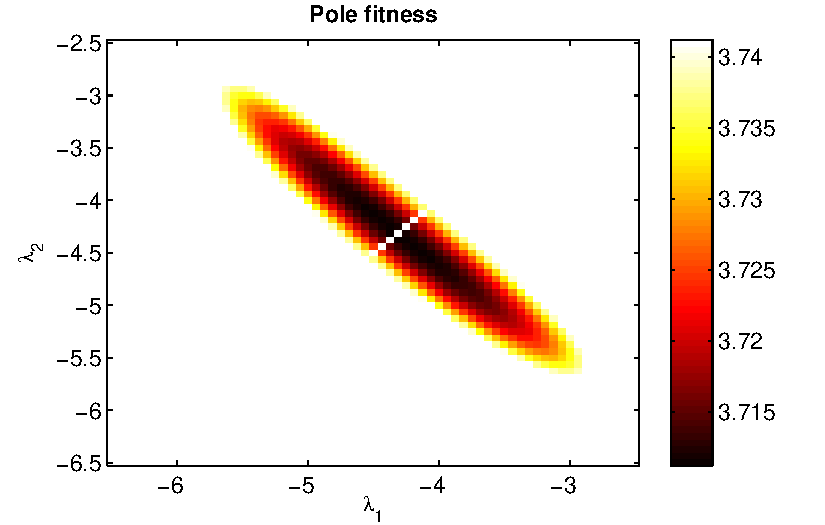
\includegraphics[width=.7\linewidth]{resource/pole-fitness.pdf}
	\end{center}
	\caption{Performance of the eigenvalues of matrix $\mat{L}$, darker means faster convergence (better)}
	\label{fig:ass2-eigs}
\end{figure}

We see the best combination of poles lies around $(-4.3; -4.4)$, so ideally we would pick these two values to calculate our eigenvalues with. The white line is there because it is not possible to have MATLAB place two equal poles. Having MATLAB \texttt{place} the given poles yields:

\begin{equation}
	\mathbf{L} =
		\begin{bmatrix}
			-7.2222 \\
			-2.0519 \\
		\end{bmatrix}.
\end{equation}

\section{Controller design}
\subsection{Oscillatory and critically-damped behavior}
In designing a controller, we want to drive KITT a to given location as fast as possible, without overshoot. This means the system should be critically damped. In this assignment, however, we are required to find a controller that introduces an oscillatory response as well. We will start by studying which behaviours can be observed when using different poles.
\\
For a general system of the form

\begin{equation*}
	\begin{split}
		\dot{\vec{x}} &= \mathbf{A}\vec{x} + \mathbf{B}\vec{u} \\
		\vec{y} &= \mathbf{C}\vec{x},
	\end{split}
\end{equation*}

we can use its Laplace-transform

\begin{equation}
	\begin{split}
		s\dot{\vec{X}}(s) &= \mathbf{A}\vec{X}(s) + \mathbf{B}\mathbf{U}(s) \\
		\vec{Y}(s) &= \mathbf{C}\vec{X}(s),
	\end{split}
	\label{eq:ass2-system-laplace}
\end{equation}

to derive an expression for $\vec{X}(s)$:

\begin{equation}
	\vec{X}(s) = (s\mathbf{I} - \mathbf{A})^{-1}\mathbf{B}\mathbf{U}(s).
	\label{eq:ass2-Xs}
\end{equation}

When substituting \ref{eq:ass2-Xs} back into \ref{eq:ass2-system-laplace}, we obtain

\begin{equation*}
	\vec{Y}(s) = \mathbf{C}(s\mathbf{I} - \mathbf{A})^{-1}\mathbf{B}\mathbf{U}(s),
\end{equation*}

which we can then use to determine the transfer function:

\begin{equation}
	\mathbf{H}(s) = \frac{\mathbf{Y}(s)}{\mathbf{U}(s)} = \mathbf{C}(s\mathbf{I} - \mathbf{A})^{-1}\mathbf{B}.
	\label{eq:ass2-Hs}
\end{equation}

It can then be shown using \ref{eq:ass2-Hs}, that for an arbitrary system $\mathbf{H}(s)$ will be of the form

\begin{equation}
	\frac{Num(s)}{Den(s)},
\end{equation}

where $Den(s)$ equals the characteristic equation of the controlled system, being $\mathrm{det}\{s\mathbf{I}-\mathbf{A})\}$. We thus notice that the poles of the system's transfer function are equal to the eigenvalues of the matrix $\mathbf{A}$. We can use this fact to determine which kind of behaviour the system will exhibit for different eigenvalues. \\
Let us write an expression for $Den(s)$ using the previous observation for a second order system:

\begin{equation}
	Den(s) = s^2 + 2\xi s \omega_n + \omega_n^2,
\end{equation}

here $\xi$ denotes the so-called \textit{damping-ratio} and $\omega_n$ is the \textit{natural frequency}. We can distinguish four different cases with respect to $\xi$:

\begin{itemize}
	\item $\xi < 0$, the poles of the system are in the right half-plane, we know this renders the system unstable
	\item $\xi > 1$, the poles of the system are real and lie in the left half-plane, the system is stable, but over-damped: it will converge slower than it could have
	\item $\xi = 1$, the system has a double pole in the right half-plane, the system is stable and critically damped: it will converge as fast as possible without overshoot
	\item $0 < \xi < 1$, the poles of the system are complex conjugates, the system is stable and under-damped: it can be shown with an inverse-Laplace-transform that it exhibits oscillatory behaviour (overshooting) and therefore converges slower
\end{itemize}
\cite{transient-systems}

\subsection{The controller itself}
Because our $\mathbf{A}$-matrix has a fixed set of poles of its own, we need a way to influence our system's characteristics (place its poles). To accomplish this, we introduce the \textit{control law} $\vec{u} = -\mathbf{K}\vec{x}$, so that the system (without observer), will be of the form

\begin{equation*}
	\begin{split}
		\dot{\vec{x}} &= (\mathbf{A}-\mathbf{B}\mathbf{K})\vec{x} \\
		\vec{y} &= \mathbf{C}\vec{x},
	\end{split}
\end{equation*}

To find a suitable matrix $K$ we can once again use MATLAB's \texttt{place}-command.
Because we want our system to converge as fast as possible, we want a critically damped response, our poles should thus be equal or at least very close to each other, since placing equal poles with MATLAB is not possible. Via trial-and-error we learned that the pair $(-1.5; -1.6)$ would yield acceptable results.
For the underdamped system we used the pair $(-1.5; -1.6)$. Both of the responses are plotted in Figure~\ref{fig:ass2-controller-response}, we see the responses we expected to see. %TODO insert actual value + K-matrices

\begin{figure}[H]
	\begin{center}
		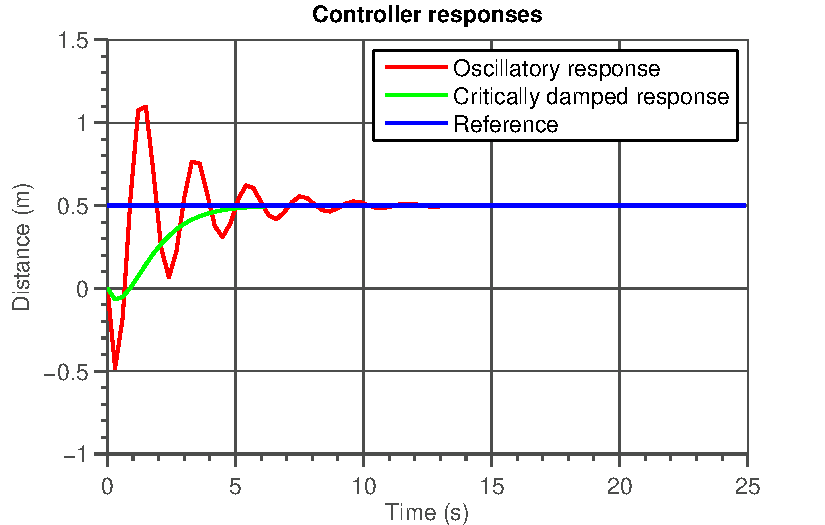
\includegraphics[width=0.7\linewidth]{resource/controller.pdf}
	\end{center}
	\caption{Oscillatory and critically damped response of the controller}
	\label{fig:ass2-controller-response}
\end{figure}

Later we learned that MATLAB implements another method of placing poles using \textit{Acker's method} (command: \texttt{acker}). This way two equal poles can be placed, which theoretically results in faster convergence. In practice, however, this improvement would most likely prove to be insignificant due to various other inaccuracies.

Finally, we want to be able to send KITT to a certain position. For this to happen, we have force KITT from his steady state to another one. We do this by applying a reference vector $\vec{r}$ to the control law, so it becomes $\vec{u} = \mathbf{K}\vec{x} + \vec{r}$. The system (without observer) is now of the form:

\begin{align}
	\dot{\vec{x}} &= (\mathbf{A}-\mathbf{B}\mathbf{K})\vec{x} + \mathbf{B}\vec{r} \\
	\vec{y} &= \mathbf{C}\vec{x}.
	\label{eq:ass2-conroller-ref}
\end{align}

When implementing this model using the previously obtained matrices, one would quickly notice it would converge to a certain state when given a reference vector $\vec{r}$ as input, but that this state would not be equal to the given reference vector. This is easily explained with the fact that we only multiply our state by $\mathbf{K}$ and consequently subtract the result from $\vec{r}$, so there is no reason to expect the state to be equal to the desired output. To overcome this issue, we must scale the reference value to be equal to the system's steady-state. Since the system is stable we can determine that $\dot{\vec{x}} \to 0$ when $t \to \infty$. Combining equations in \ref{eq:ass2-conroller-ref} then yields

\begin{equation}
	\vec{y} \to \mathbf{C} (\mathbf{B} \mathbf{K} - \mathbf{A})^{-1} \mathbf{B} \vec{r} \text{ when } t \to \infty.
\end{equation}

When multiplying the reference vector with the inverse of the above result, the system will converge to the desired state. The complete and final system then becomes

\begin{equation}
	\dot{\hat{\vec{x}}} = (\mathbf{A}-\mathbf{L}\mathbf{C}-\mathbf{B}\mathbf{K}) \hat{\vec{x}} + \mathbf{B}(\mathbf{C}(\mathbf{B} \mathbf{K} - \mathbf{A})^{-1} \mathbf{B})^{-1} \vec{r} + \mathbf{L} \vec{y}.
\end{equation}

Alas, there is one last issue to deal with. The given model is for continuous time, where we read KITT's output at a pretty low rate. Therefore the model must be discretized for approximating the current state at discrete intervals. To do this we used Heun's method, which gives an estimation of the next state by averaging the current slope and a predicted next slope. \cite{wikipedia-heuns}

\section{Considerations}
There are a few things that set our theoretically fine model aside from reality. \\
A big hit on the accuracy of the controller is the fact that the connection's latency when requesting the current state can increase up to \SI{600}{ms}. In this time a lot can happen, especially when KITT is driving fast, so severe overshoot is not uncommon. We think this lag is due to MATLAB, so because we have an implementation of the model in both Python and C\# ready for testing, we hope this lag will decrease to more acceptable levels in the future. \\
Another issue is the dependency of KITT's performance on the current battery voltage. The lower that gets, the slower KITT will be. The model itself does not implement this property, so it might be worth implementing some form of compensation ourselves. \\
There is also the fact that the sensors sometimes output incorrect values, even though we filter these before using them in the model, sometimes a spike gets through. \\
And lastly, of course some inaccuracy is caused by the model being only a linearly fitted approximation of reality. \\

\section{Controlling KITT}
Every non-ideality we discussed aside, we were able to control KITT in some degree. Plots of KITT's response are shown in Figure~\ref{fig:ass2-kitt-controlled}. The clamped output was introduced to reduce KITT's maximum speed for preventing accidents and monumental overshoot. We see that KITT slowly drives towards the reference value, which is an accomplishment.

\begin{figure}[H]
	\begin{subfigure}{.5\textwidth}
		\centering
		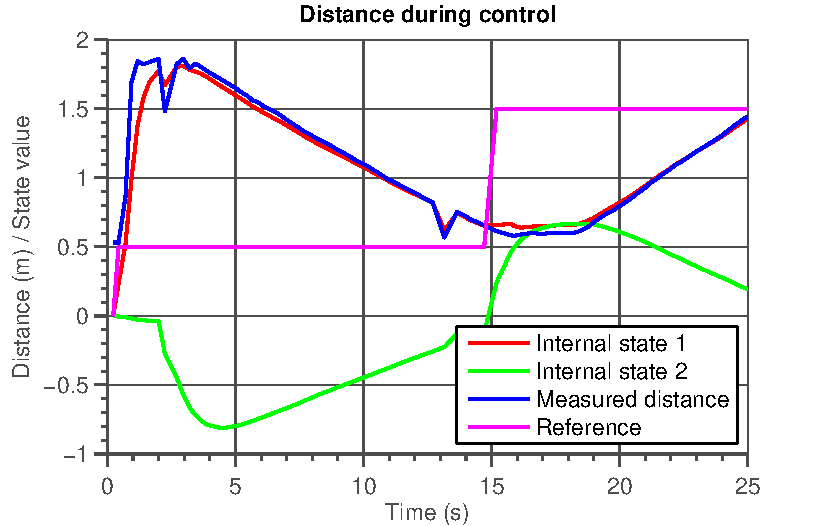
\includegraphics[width=\linewidth]{resource/measurement-states.pdf}
		\caption{Internal states, measured distance and reference during control}
	\end{subfigure}
	\begin{subfigure}{.5\textwidth}
		\centering
		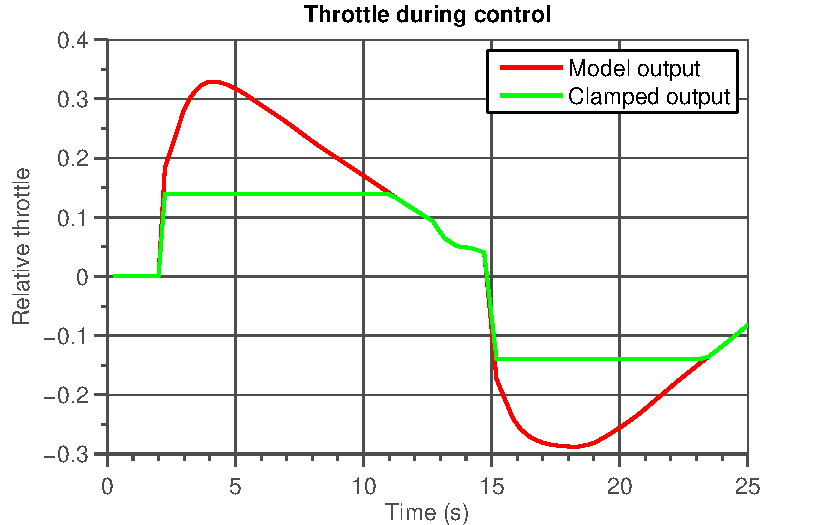
\includegraphics[width=\linewidth]{resource/measurement-drive.pdf}
		\caption{Relative throttle during control}
	\end{subfigure}
	\caption{Measurement results of KITT controlled by the designed controller}
	\label{fig:ass2-kitt-controlled}
\end{figure}

Without MATLAB and with some more optimizations, we hope things will get better.

\end{document}